\documentclass[11pt]{article}
\title{Meccano hexagons gallery}
\author{https://github.com/heptagons/meccano/hexa/gallery}
\date{2023/12/27}

\usepackage{../../meccano}
\usepackage{amssymb}
\usepackage{subcaption}


\begin{document}

\maketitle
\begin{abstract}
We build meccano\meccanoref rigid regular heptagons.
\end{abstract}

\section{Heptagon internals}

\begin{figure}[h]
\centering
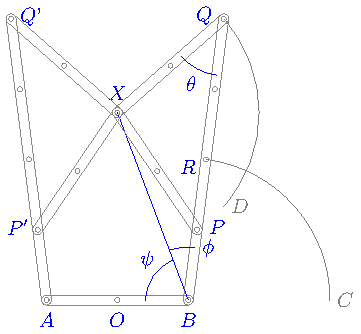
\includegraphics[scale=0.9]{builder/hepta-base}
\caption{Cluster with fixed vertices $A=(-1,0)$, $B=(+1,0)$, $X=(0,\sqrt7)$ useful to build a regular heptagon.}
\label{fig:build-base}
\end{figure}

Figure \ref{fig:build-base} show a cluster to make a triangle $\triangle{ABX}$ useful to make a regular heptagon. With the law of cosines we calculate first the angle $\theta \equiv \angle{PQX}$ and then the distance $\overline{BX}$:
\begin{align}
\cos\theta &= \frac{(\overline{PQ})^2 + (\overline{QX})^2 - (\overline{XP})^2}
 {2(\overline{PQ})(\overline{QX})} 
 = \frac{3^2 + 2^2 - 2^2}{2(3)(2)} = \frac{3}4 \\
\overline{BX} &= \sqrt{(\overline{BQ})^2 + (\overline{QX})^2 
 - 2(\overline{BQ})(\overline{PQ})\cos\theta}
 = \sqrt{4^2 + 2^2 - 2(4)(2)\left(\frac{3}4\right)} = 2\sqrt2
\end{align}

Since $\overline{AX} = \overline{BX}$ triangle $\triangle{ABX}$ is isoscelles and we calculate $\overline{OX}$:
\begin{align}
\overline{OX} &= \sqrt{(\overline{BX})^2 - (\overline{OB})^2}
 = \sqrt{(2\sqrt2)^2 - 1^2} = \sqrt7
\end{align}

\begin{figure}[h]
\centering
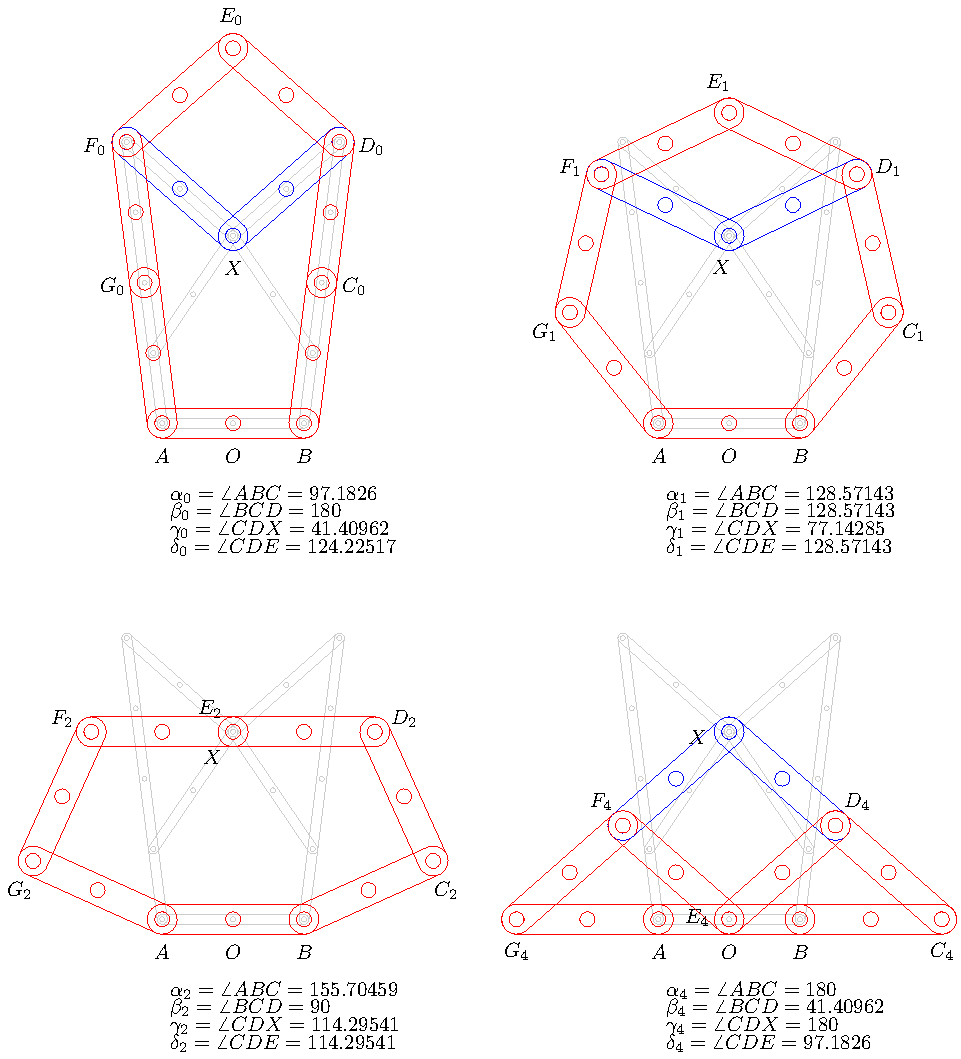
\includegraphics[scale=0.9]{builder/hepta-0}
\caption{Equilateral heptagons connected to rigid triangle $\triangle{ABX}$.}
\label{fig:build}
\end{figure}

Figure \ref{fig:build} show equilateral heptagons $ABCDEFG$ connected to the cluster of figure \ref{fig:build-base}. The heptagon has two internal strips $\overline{DX}$ and $\overline{FX}$ and vertices $A$, $B$ and $X$ are fixed. We move the strips symmetrically. In figure $(a)$ we have the maximum extension to the top limited by fact that vertices $B$ and $D_0$ cannot be separated more since both are collinear with vertice $C_0$, being the angle $\beta_0 = \pi/2$. From $(a)$ we reach state $(b)$ reducing $\beta$ until $\alpha_1 = \beta_1 = \delta_1 = 3\pi/7$ the regular heptagon. From $(b)$ we reach state $(c)$ reducing $\beta$ until $\beta= \pi/2$. In figure $(d)$ we reach the maximum extension to the bottom limited by the fact that vertices $X$ and $C_3$ cannot be separated more since both are collinear with vertice $D_3$, being the angle $\beta_3 = acos(3/4)$.

\end{document}
